\section{Even More Functions}

    \subsection{Monotonic Functions}
        \textbf{Monotonicity} refers to intervals of increase and decrease.
        \textbf{Monotonic Functions} are functions that are strictly increasing or strictly
        decreasing on their entire domains. \\

        \begin{center}
            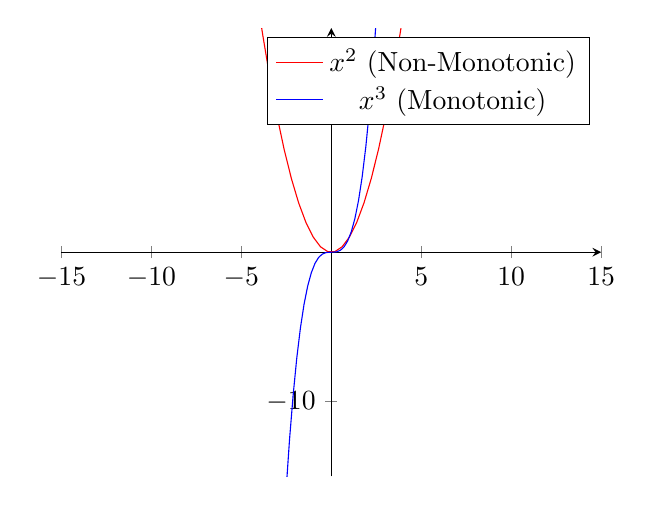
\begin{tikzpicture}
                \begin{axis}[
                    axis lines = center,
                    xmin = -15,
                    xmax = 15,
                    ymin = -15,
                    ymax = 15,
                ]
                % x^2
                \addplot [
                    domain=-20:20,
                    samples=100,
                    color=red,
                ]
                {x^2};
                \addlegendentry{$x^2$ (Non-Monotonic)}
                % x^3
                \addplot [
                    domain=-10:10,
                    samples=100,
                    color=blue,
                ]
                {x^3};
                \addlegendentry{$x^3$ (Monotonic)}
                \end{axis}
            \end{tikzpicture}
        \end{center}



    \subsection{Even and Odd Functions}
        \textbf{Even functions} $(f(-x)=f(x))$ are unchanged when reflected across the y-axis.
        \textbf{Odd functions} $(f(-x)=-f(x)$ are unchanged when rotated $180\degree$ about the origin. \\

        \begin{center}
            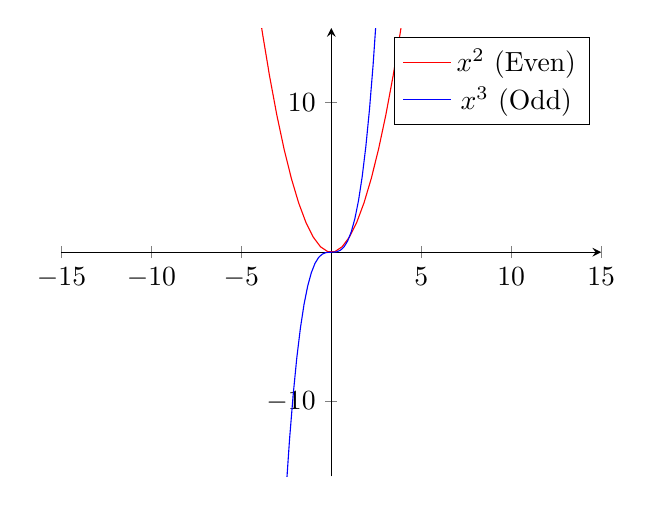
\begin{tikzpicture}
                \begin{axis}[
                    axis lines = center,
                    xmin = -15,
                    xmax = 15,
                    ymin = -15,
                    ymax = 15,
                ]
                % x^2
                \addplot [
                    domain=-20:20,
                    samples=100,
                    color=red,
                ]
                {x^2};
                \addlegendentry{$x^2$ (Even)}
                % x^3
                \addplot [
                    domain=-10:10,
                    samples=100,
                    color=blue,
                ]
                {x^3};
                \addlegendentry{$x^3$ (Odd)}
                \end{axis}
            \end{tikzpicture}
        \end{center}



    \subsection{Piecewise and Parametric Functions}
        Functions that are defined differently across its $x$-intervals are
        \textbf{piecewise functions}. Consider the function defined below \\

        \begin{equation*}
            f(x)=
            \begin{cases}
                x^2 & ,x<2 \\
                6 & ,x=2 \\
                10-x & , 2<x\leq 6
            \end{cases}
        \end{equation*}

        \noindent The domain is then $\{x\in\mathbb{R}|x\leq 6\}$ and the graph looks like this: \\

        \begin{center}
            \begin{tikzpicture} [circ/.style={circle,draw,inner sep=2pt}]
                \begin{axis}[
                    axis lines = center,
                    xmin=-4.5,
                    xmax=6.5,ymin=-2,
                    xlabel={$x$},ylabel={$y$},
                ]
                %f(x), x < 2
                \addplot [
                    red,
                    smooth,
                    {Stealth[bend]}-,
                    domain=-4:2,
                    postaction={decoration={text along path,
                    text align={align=center},
                    text={|\color{red}|{$y$}{${}={}$}{${x^2}$}},
                    raise=-2.5ex,
                    },
                    decorate}
                ]
                {x^2}
                node[pos=1,circ,fill=white]{};
                \addlegendentry{$f(x)$}
                %f(x), x = 2
                \path (2,6) node [
                    circ,
                    fill=red!60
                ]
                {};
                %f(x), 2 < x <= 6
                \addplot [
                    red,
                    samples=2,
                    domain=2:6
                ]
                {10-x};
                node[pos=0,circ,fill=white]{};
                node[pos=1,circ,fill=red!60]{};
                \end{axis}
            \end{tikzpicture}
        \end{center}

        \noindent Instead of defining a single function $y=f(x)$, \textbf{Parametric Equations} are
        defined as multiple functions together, one for each variable. Hence, we can represent a
        function with $x$ and $y$ in terms of the \textbf{parameter} $t$ as below:

        \begin{center}
            \begin{tabular} {cc}
                $x=f(t)$ & $y=g(t)$
            \end{tabular}
        \end{center}

        \noindent An example of a \textbf{parametric curve}, the set of points the parameter gives
        in all the parametric equations, is the parent circle given by $x^2+y^2=r^2$. Isolating $x$
        and $y$ give our two parametric equations, $y=\pm\sqrt{r^2-x^2}$ and $x=\pm\sqrt{r^2-y^2}$. \\

        \noindent When we sketch parametric curves, we plug in values of the parameter and find
        their x and y-values, graphing each point of the form $(x,y)$ on the Cartesian Plane.
        It is important to note that parametric curves always have a \textbf{direction of motion},
        represented by arrows on the curve given by the increasing parameter $t$.

        \noindent We can \textbf{eliminate the parameter} from a set of parametric equations by
        solving for the parameter $t$ in one of the equations and plugging the value for $t$ into
        the second parametric equation.\\

        \begin{figure} [hbt!]
            \centering
            \includegraphics [scale = 0.5] {Resources/Unit9EvenMoreFunctions/param.png}
        \end{figure}



    \subsection{The Absolute Value Function}
        An \textbf{Absolute Value Function} is a function involving absolute value operations.
        The absolute value parent function is \\

        \begin{equation*}
            f(x)=|x|=
            \begin{cases}
                x, & x>0 \\
                0, & x=0 \\
                -x, & x<0
            \end{cases}
        \end{equation*}

        \noindent Absolute value functions are V-shaped and to graph them we simply choose some
        $x$-values and plot their ordered pairs. \\

        \begin{center}
            \begin{tikzpicture}
                \begin{axis}[
                    axis lines = center,
                    xmin = -5,
                    xmax = 5,
                    ymin = -5,
                    ymax = 5
                ]
                % f(x)
                \addplot [
                    samples=100,
                    color=red,
                ]
                {abs(x)};
                \addlegendentry{$f(x)=|x|$}
                \end{axis}
            \end{tikzpicture}
        \end{center}



    \subsection{The Floor and Ceiling Functions}
        The \textbf{floor} of a number is the nearest integer down. The \textbf{ceiling} of a number
        is the nearest integer up. For 2.31, the floor is 2 and the ceiling is 3. The floor and
        ceiling of integers are the integers themselves. The floor of $x$ is represented by
        $\floor*{x}$ and the ceiling by $\ceil*{x}$. \\

        \noindent The \textbf{Floor Function} is piecewise, discontinuous at each integer, and is
        composed of the greatest integer that is less than or equal to $x$. The
        \textbf{Ceiling Function} is piecewise, discontinuous at each integer, and is composed of
        the least integer that is greater than or equal to $x$.\\

        \noindent \color{purple} \textbf{Properties of Floor and Ceiling Functions:} \color{black} \\
        1. $\floor*{x+n}=\floor*{x}+n$ for any integer $n$ \\
        2. $\floor*{x}+\floor*{-x}=\begin{cases}
                                       -1, & x \not\in \mathbb{Z}\\0, &x\in\mathbb{Z}
        \end{cases}$ \\
        3. $\floor*{x+y}=\floor*{x}+\floor*{y}=\floor*{x}+\floor*{y}+1$ \\

        \noindent Similary, all of the floor brackets can be replaced with ceiling brackets for
        their properties as well. \\

        \noindent The domain of the floor function is given by $\floor*{x}\leq x<\floor*{x}+1$. \\

        \noindent \color{blue} \textit{Example 1: Find all the values of $x$ that satisfy
        $\floor*{0.5+\floor*{x}}=20$}. \color{black} \\
        Let $y=\floor*{x}$. Then \\

        \begin{align*}
            \floor*{0.5+y} &= 20 \\
            & \iff \\
            20\leq y &+ 0.5 <21\\
            19.5\leq &y <20.5
        \end{align*}

        \noindent Since $y$ is an integer and $y=20$ is the only interval in this interval,
        this becomes $y=20=\floor*{x}$. Since any value less than 21 and greater than or equal to
        20 wil satisfy this equation, the answer is $\{x\in\mathbb{R}|20\leq x<21\}$. \\

        \begin{center}
            \begin{tikzpicture} [circ/.style={circle,draw,inner sep=1.5pt}]
                \begin{axis} [
                    axis lines = center,
                    xmin = -5,
                    xmax = 5,
                    ymin = -5,
                    ymax = 5,
                    xlabel={$x$},ylabel={$y$},
                ]
                %Floor function
                \addplot[red,samples=2,domain=-4:-3] {-4}
                    node[pos=0,circ,fill=red!60]{}
                    node[pos=1,circ,fill=white]{};
                \addplot[red,samples=2,domain=-3:-2] {-3}
                    node[pos=0,circ,fill=red!60]{}
                    node[pos=1,circ,fill=white]{};
                \addplot[red,samples=2,domain=-2:-1] {-2}
                    node[pos=0,circ,fill=red!60]{}
                    node[pos=1,circ,fill=white]{};
                \addplot[red,samples=2,domain=-1:0] {-1}
                    node[pos=0,circ,fill=red!60]{}
                    node[pos=1,circ,fill=white]{};
                \addplot[red,samples=2,domain=0:1] {0}
                    node[pos=0,circ,fill=red!60]{}
                    node[pos=1,circ,fill=white]{};
                \addplot[red,samples=2,domain=1:2] {1}
                    node[pos=0,circ,fill=red!60]{}
                    node[pos=1,circ,fill=white]{};
                \addplot[red,samples=2,domain=2:3] {2}
                    node[pos=0,circ,fill=red!60]{}
                    node[pos=1,circ,fill=white]{};
                \addplot[red,samples=2,domain=3:4] {3}
                    node[pos=0,circ,fill=red!60]{}
                    node[pos=1,circ,fill=white]{};
                \end{axis}
            \end{tikzpicture} \\
            \textbf{The Floor Function}
        \end{center}

        \begin{center}
            \begin{tikzpicture} [circ/.style={circle,draw,inner sep=1.5pt}]
                \begin{axis}[
                    axis lines = center,
                    xmin = -5,
                    xmax = 5,
                    ymin = -5,
                    ymax = 5,
                    xlabel={$x$},
                    ylabel={$y$}
                ]
                %Ceiling function
                \addplot[red,samples=2,domain=-4:-3] {-4}
                    node[pos=0,circ,fill=white]{}
                    node[pos=1,circ,fill=red!60]{};
                \addplot[red,samples=2,domain=-3:-2] {-3}
                    node[pos=0,circ,fill=white]{}
                    node[pos=1,circ,fill=red!60]{};
                \addplot[red,samples=2,domain=-2:-1] {-2}
                    node[pos=0,circ,fill=white]{}
                    node[pos=1,circ,fill=red!60]{};
                \addplot[red,samples=2,domain=-1:0] {-1}
                    node[pos=0,circ,fill=white]{}
                    node[pos=1,circ,fill=red!60]{};
                \addplot[red,samples=2,domain=0:1] {0}
                    node[pos=0,circ,fill=white]{}
                    node[pos=1,circ,fill=red!60]{};
                \addplot[red,samples=2,domain=1:2] {1}
                    node[pos=0,circ,fill=white]{}
                    node[pos=1,circ,fill=red!60]{};
                \addplot[red,samples=2,domain=2:3] {2}
                    node[pos=0,circ,fill=white]{}
                    node[pos=1,circ,fill=red!60]{};
                \addplot[red,samples=2,domain=3:4] {3}
                    node[pos=0,circ,fill=white]{}
                    node[pos=1,circ,fill=red!60]{};
                \end{axis}
            \end{tikzpicture} \\
            \textbf{The Ceiling Function}
        \end{center}



    \subsection{The Fractional Part Function}
        The \textbf{Fractional Part Function} is defined as $f(x)=\{x\}=x-\floor*{x}$.
        For nonnegative real numbers, the fractional part is simply the part after the decimal.
        For example, $\{3.64\}=3.64-\floor*{3.64}=3.64-3=0.64$. \\

        \noindent \textbf{Properties of the Fractional Part Function:} \\
        1. $0\leq\{x\}<1$ and $0=\{x\}$ if and only if $x$ is an integer \\
        2. $\{x\}+\{-x\}=$

        \begin{cases}
            0 & \text{if } x \text{ is an integer} \\
            1 & \text{otherwise}
        \end{cases}

        \noindent 3. If $a$ and $b$ are integers and $b>0$ then $\{\frac{a}{b}\}=\frac{r}{b}$, where
        $r$ is the remainder from dividing $a$ by $b$.

        \begin{center}
            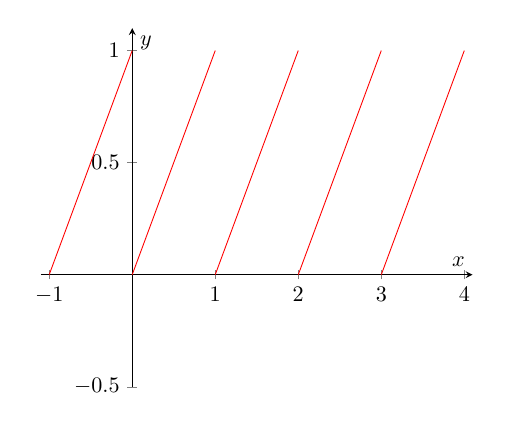
\begin{tikzpicture}[circ/.style={circle,draw,inner sep=1.5pt}, scale = 0.8]
                \begin{axis}[
                    axis lines = center,
                    xmin = -1.1,
                    xmax = 4.1,
                    ymin = -0.5,
                    ymax = 1.1,
                    xlabel={$x$},
                    ylabel={$y$}
                ]
                %Coordinates
                \coordinate (A) at (-1,0);
                \coordinate (B) at (0,1);
                \coordinate (C) at (0,0);
                \coordinate (D) at (1,1);
                \coordinate (E) at (1,0);
                \coordinate (F) at (2,1);
                \coordinate (G) at (2,0);
                \coordinate (H) at (3,1);
                \coordinate (I) at (3,0);
                \coordinate (J) at (4,1);
                %%%
                %Functions
                \draw[color=red] (A) -- (B);
                \draw[color=red] (C) -- (D);
                \draw[color=red] (E) -- (F);
                \draw[color=red] (G) -- (H);
                \draw[color=red] (I) -- (J);
                %%%
                \end{axis}
            \end{tikzpicture} \\
            \textbf{The Fractional Part Function}
        \end{center}